\subsection{Validazione e Collaudo}
Dal 2020-04-21 al 2020-05-17\\
Inizia al termine della fase di Progettazione di Dettaglio e Codifica e finisce con la data di consegna per la Revisione di Accettazione.\\
In questo fase vengono definite le attività che servono a verificare che il prodotto corrisponda a quello desiderato dal committente e dal proponente.

\subsubsection{Periodo 1} 
Dal 2020-04-21 al 2020-04-28
\begin{itemize}
	\item \textbf{Normazione}: Standardizzazione e correzione di alcune parti della documentazione che non aderiscono completamente alle \NdP{};
	\item \textbf{Correzioni}: Correzioni di difetti notati dal committente (ove presenti) nella \glo{Product Baseline};
	\item \textbf{Assegnazione dei ruoli di progetto}: Assegnazione dei ruoli di ciascun membro del gruppo in base alla suddivisione oraria indicata in §5.4.1;
	\item \textbf{Soddisfazione dei requisiti}: Controllo che i requisiti siano soddisfatti;
	\item \textbf{Pianificazione attività}: Le attività da svolgere devono essere prima pianificate e discusse dal gruppo per garantire il \glo{way of working} sancito nelle \NdP{};
	\item \textbf{Verifica}: \glo{Verifica} dell'andamento del gruppo in relazione alle tempistiche e allo svolgimento dei compiti assegnati.
\end{itemize}

\subsubsection{Periodo 2} 
Dal 2020-04-29 al 2020-05-10
\begin{itemize}
	\item \textbf{Codifica}: Esecuzione dell'ultimo versionamento del prodotto;
	\item \textbf{Verifica}: Accertamento che le esecuzioni delle attività siano esenti da errori (condizione necessaria ma non sufficiente: superamento dei test di unità, di integrazione, di sistema);
	\item \textbf{Validazione}: Verifica se il prodotto realizzato sia conforme alle attese, e validazione finale in caso di esito positivo;
	\item \textbf{Scrittura dei manuali}: Esecuzione del secondo versionamento del Manuale Utente e del Manuale Manutentore;
	\item \textbf{Collaudo}: Vengono eseguiti gli ultimi test sul prodotto per verificare se le funzionalità rispettano i risultati attesi.
\end{itemize}

\subsubsection{Periodo 3} 
Dal 2020-05-11 al 2020-05-17
\begin{itemize}
	\item \textbf{Preparazione per la Revisione di Accettazione}: Il gruppo produce il materiale necessario da esporre alla presentazione pubblica della propria proposta.
\end{itemize}

%PAGINA ORIZZONTALE
\newpage
\paperwidth=\pdfpageheight
\paperheight=\pdfpagewidth
\pdfpageheight=\paperheight
\pdfpagewidth=\paperwidth
\headwidth=\textheight

\begingroup 
\vsize=\textwidth
\hsize=\textheight

\subsubsection{Diagramma di Gantt delle attività di Validazione e Collaudo}
\pagestyle{empty}
\begin{figure}[h]
	\centering
	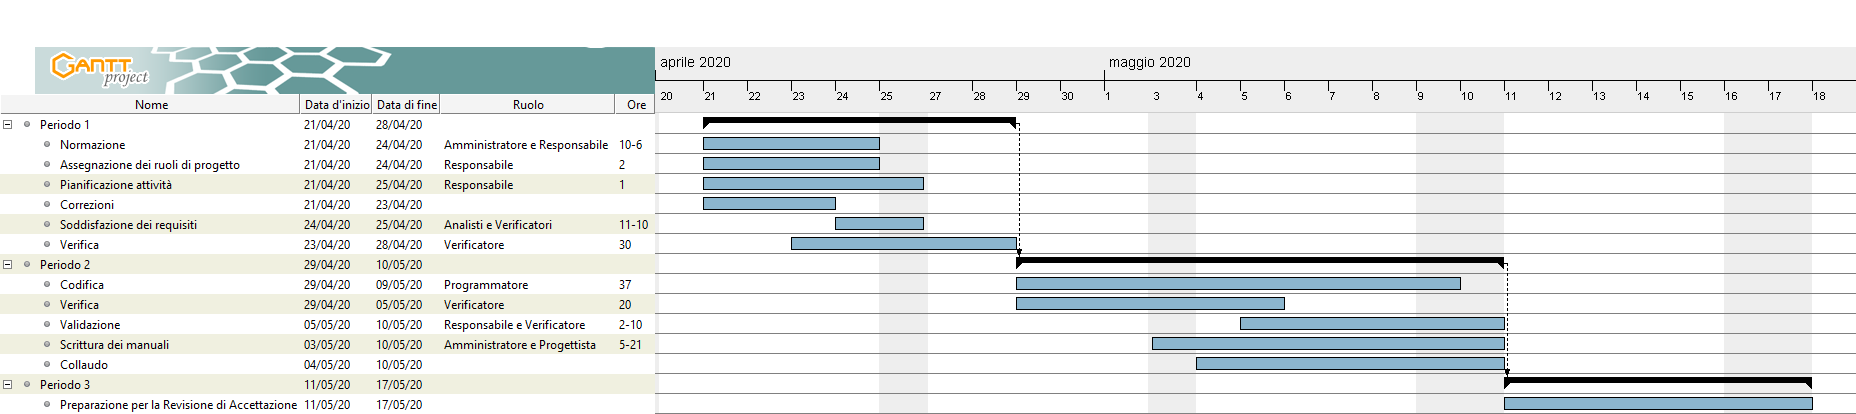
\includegraphics[scale=0.40]{Sezioni/DiagrammiGantt/Validazione.png}
	\caption{Diagramma di Gantt delle attività di Validazione e Collaudo}
\end{figure}

\textwidth=\hsize
\textheight=\vsize

\endgroup
\newpage
\paperwidth=\pdfpageheight
\paperheight=\pdfpagewidth
\pdfpageheight=\paperheight
\pdfpagewidth=\paperwidth
\headwidth=\textwidth